%%=============================================================================
%% Inleiding
%%=============================================================================

\chapter{Inleiding}
\label{ch:inleiding}

Het doel van de bachelorproef is om blockchain toe te passen op het werk dat een verzekeringsmakelaar verricht, dus het beveiligen van unieke documenten zoals verzekeringsdocumenten en voorkomen om documenten te vervalsen of dubbele schadeclaims te verrichten. Bovendien willen we ook streven naar een betere uniformiteit en communicatie tussen verschillende partijen. Dit is dan meteen ook onze usecase.

\section{Blockchain}
\label{sec:stand-van-zaken}

%% TODO: deze sectie (die je kan opsplitsen in verschillende secties) bevat je
%% literatuurstudie. Vergeet niet telkens je bronnen te vermelden!`

\subsection{Wat is blockchain?}

Blockchain is een technologie die het best kan vergeleken worden met een database. Het wordt dan ook vooral gebruikt om gevoelige data veilig op te slaan. Blockchain dook voor het eerst op in het Bitcoin whitepaper door \textcite{Nakamoto2008}, dit blijkt een alias te zijn voor een persoon of een groep en de echte ontwikkelaar is niet gekend bij naam. Uit dit document kan afgeleid worden dat het gaat om een enkel persoon maar dit is niet met zekerheid geweten. 

 Blockchain is een peer-to-peer technologie of ook ``ledgers'' genoemd. Dit wil zeggen dat alle data niet in één plaats is opgeslagen maar op verschillende servers of ook nodes genoemd. Zo heeft elke node een versie van de blockchain. Dit is meteen ook één van de reden waarom blockchain zo veilig is en ook niet eenvoudig is om te hacken, bovendien is de blockchain volledig geëncodeerd door middel van een hash, deze verwijst naar de vorige blok en de volgende blok. Een voorbeeld van de hash is te zien in op figuur \ref{fig:blockchain-hash-example}. Hoe veilig deze technologie juist is wordt uitgelegd in een volgend hoofdstuk.
 
 Blockchain is meteen ook de technologie achter het bekende Bitcoin. Het idee was om digitaal geld te kunnen transporteren van één partij naar een andere zonder de tussenkomst van een financiële instelling of dergelijke. Blockchain heeft dan ook het grote voordeel te werken met een peer-to-peer systeem wat waarschijnlijk raar klinkt voor een geld transport systeem aangezien banken werkten met een centraal systeem om veiligheid te garanderen. Dit heeft uiteraard ook vele nadelen zoals het integreren met andere platformen. Toch blijkt blockchain een veilige manier te zijn en dit door de manier van hoe blockchain werkt.
 
 Blockchain het makkelijkst voorstellen als een excel-blad. Elke rij in het blad is een transactie, en de transactie heeft telkens een relatie met de vorige transactie. Dit is te zien op figuur \ref{fig:blockchain-transaction-example}. Zo kan er dus bijvoorbeeld geen 10.000 euro getoverd worden op een bitcoin rekening aangezien deze moet gestort worden met een transactie en dus wel degelijk ergens vandaan moet komen.
 
 \begin{figure}
 	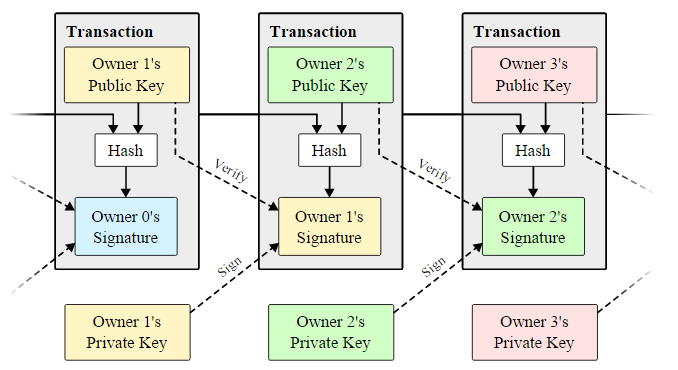
\includegraphics[width=\linewidth]{blockchaintransactions.png}
 	\caption{Voorbeeld van transacties. Bron: \textcite{Nakamoto2008} }
 	\label{fig:blockchain-transaction-example}
 \end{figure}
\begin{figure}
	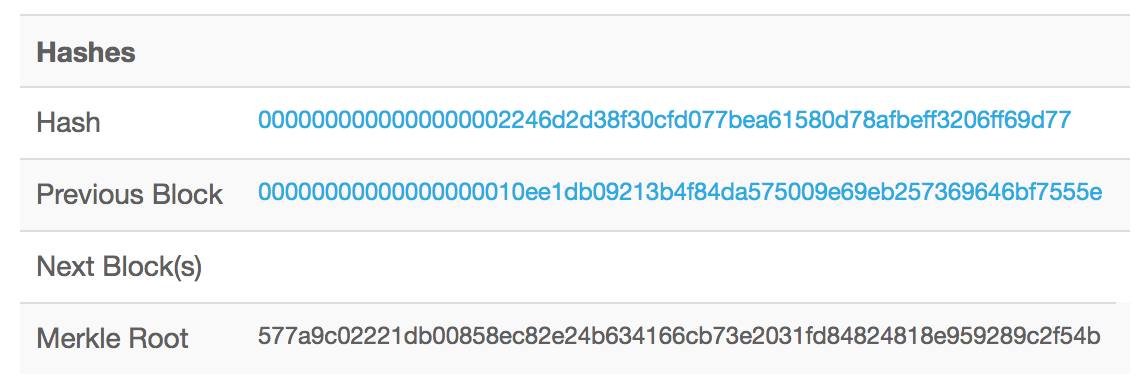
\includegraphics[width=\linewidth]{blockchain-hashes.png}
	\caption{Voorbeeld van hashes. Bron: \textcite{blockchain.info}}
	\label{fig:blockchain-hash-example}
\end{figure}

 \subsubsection{Hoe wordt een blockchain geïnitialiseerd?}
Natuurlijk moet er wel een manier zijn om bijvoorbeeld nieuw geld in de blockchain toe te voegen, dit moet dan uiteraard wel ergens vandaan komen dus er moet natuurlijk wel een manier zijn om instanties aan te kunnen maken. 

De eerste transactie in een blok wordt gezien als een speciale transactie die meteen ook een nieuwe munt zal aanmaken waar hij eigenaar van is. Dus voor elke eerste transactie van een blok wordt een nieuwe munt aangemaakt waarvan de node dus eigenaar is. Dit zorgt meteen ook voor een goed motief om het netwerk van nodes te steunen en zorgt ook meteen voor een manier om nieuwe munten in omloop te brengen aangezien er geen centrale authoriteit is die de blockchain beheert. 

Er wordt dus constant geld toegevoegd aan de bitcoin blockchain door het gevolg van het verbruiken van middelen. In het geval van Bitcoin is dit bijvoorbeeld elektriciteit en CPU-kracht en dit zal voor de meeste blockchains ook het geval zijn. Dus met andere woorden wordt het openstellen van CPU-kracht en het gebruik hiervan beloond door het verkrijgen van bitcoins bij het aanmaken van een nieuw blok. Dit heeft ook als voordeel dat het proberen hacken van de blockchain niet meer zo gunstig zou zijn en het dus beter is om een ``eerlijke'' node te blijven. Natuurlijk is het niet nodig om steeds een nieuwe munt aan te maken als motivatie want dit zou zorgen voor inflaties. Wanneer er bijvoorbeeld een genoeg aantal munten in omloop zijn kan het gehele systeem van verbruikte middelen ook vergoed worden door transactiekosten zodat er helemaal geen inflatie optreedt.

\subsection{Kan iedereen zich aansluiten bij de nodes?}
Iedereen kan lid worden van een blockchain netwerk en CPU-kracht beschikbaar stellen wanneer de blockchain publiek is zoals dit bij Bitcoin het geval is, dit wordt ook ``gold miners'' genoemd in de Bitcoin blockchain. Een eigen computer ter beschikking stellen als node in het netwerk is mogelijk waardoor de gebruiker vergoed wordt met bitcoins. Deze zouden dan ook de kosten moeten dekken van de elektriciteit en de verbruikte CPU-kracht. Wie dus CPU-kracht over heeft kan deze ter beschikking stellen en hier aan verdienen. Op deze manier probeert  bitcoin bijvoorbeeld ook om alle nodes ``eerlijk'' te houden aangezien dit veel interessanter zou zijn. Het opstellen van een gold miner wordt later uitgelegd. 

Tegenwoordig kan dit niet meer door een eigen computer ter beschikking te stellen voor Bitcoin aangezien de verloning voor elektriciteit en CPU-kracht te laag zou zijn om dit competetief te houden. Daarom is er tegenwoordig hardware te koop om Bitcoins te minen (het verdienen van bitcoins) die gemaakt zijn speciaal hiervoor. Deze zijn meteen ook veel zuiniger. Dit volgens het volgende artikel \textcite{Bitcoinmining.com}.
 
\subsection{Soorten in blockchain}

\begin{figure}
	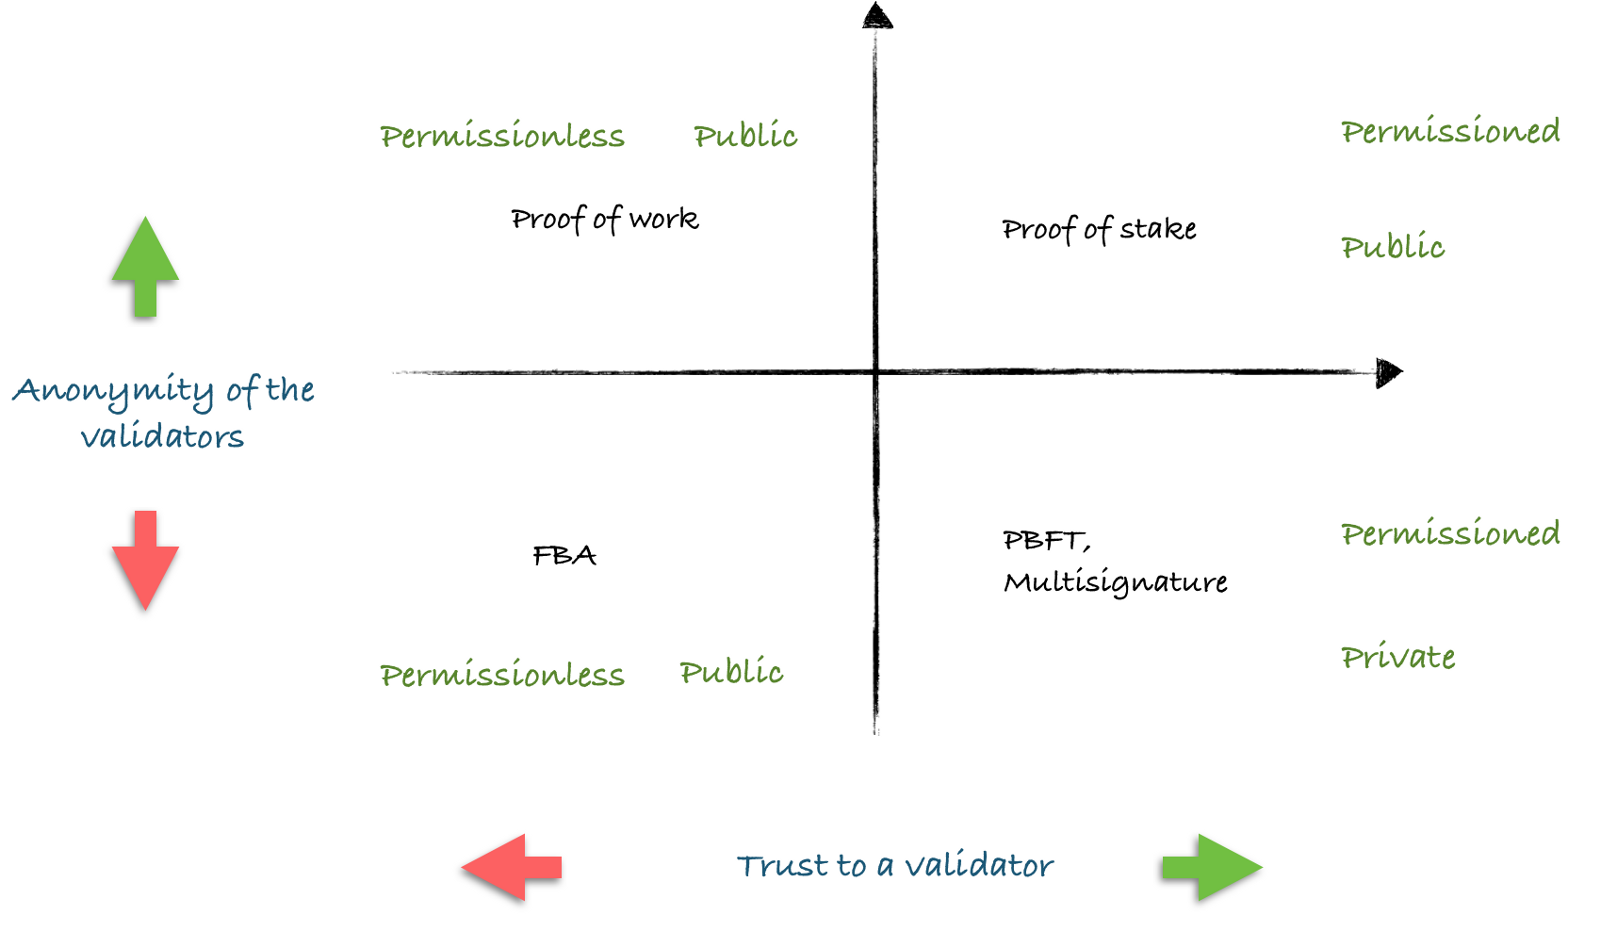
\includegraphics[width=\linewidth]{blockchain-types.png}
	\caption{Grafische voorstelling van enkele varianten van de blockchain types die bestaan. Enderzijds publieke versus private en anderzijds met rechten of zonder rechten. Bron: \textcite{Kravchenko2016}}
	\label{fig:blockchain-types}
\end{figure}

Natuurlijk zijn er verschillende soorten blockchain. Doorheen de literatuurstudie wordt telkens Bitcoin als voorbeeld gebruikt, Bitcoin is uiteraard een publiek netwerk waar geen rechten op toegekend waren. Dit volgens \textcite{Nakamoto2008}. Natuurlijk is dit niet de enige soort en zijn er nog andere varianten die telkens toch wat verschillen hebben. Hoofdzakelijk zijn er 2 veranderlijken, de anonimiteit en de hoeveelheid vertrouwen die de gebruiker heeft. \textcite{Kravchenko2016} maakte hierover een uitgebreid artikel en gebruikte het volgende schema dat te zien is op Figuur \ref{fig:blockchain-types}.

Wie zien meteen dat Blockchain bovenaan links in de groep hoort. Niemand is gekend op het netwerk, er zijn geen rechten van toepassing en iedereen heeft toegang. De enige manier van validatie die hier van toepassing is, is proof-of-work. Men moet dus nooit op voorhand hebben deelgenomen of doorgelicht geweest zijn om deel te kunnen nemen. Het vertrouwen dat aan een ``miner'' (een node wordt bij bitcoin ook een miner genoemd) wordt gegeven is laag en er is ook geen straf voor het aanvallen van het systeem buiten het feit dat de mining apparatuur (hardware die geschikt is om gebruikt te worden als node) niet verder kan gebruikt worden als de aanval succesvol was. Dit type is dus vooral geschikt voor volledig anonieme systemen die volledig buiten een overheidinstanties werken. 

Bovenaan rechts is een publieke blockchain maar deze keer wel met rechten. Dit omdat er munten moeten gekocht worden om te kunnen minen. Een munt is dan ook iets wat van het systeem zelf is en niet werkt zoals Bitcoin waar een munt wordt gegeven aan de eigenaar van mining machines. Deze soort beveiliging wordt ook ``proof of stake'' genoemd. Dit soort systemen geven hierdoor ook meer vertrouwen aan de gebruiker aangezien bij een aanval op het syteem de ``borg'' verloren gaat bij het proberen uitvoeren van een aanval of dubbele uitgave. Dit soort systemen is ideaal voor de uitvoering van contracten, gemeenschapsbestuur, privé geld systemen, enz. 

Onderaan links bevindt zich de privé blockchain zonder regels. Onder bepaalde sociale overeenkomsten kan iedereen toegang krijgen tot het syteem en dus een node worden in het systeem. Een goed voorbeeld hiervan is bijvoorbeeld een land waar elke bewoner het recht heeft om een node te worden van het netwerk. Het vertrouwen dat wordt gegeven aan een node is vrij laag, zelfs met de identiteit die gekend is. Dit is meteen ook een groot verschil met de bitcoin variant waar iedereen niet gekend is. Hoe komen systemen dan overeen bij validatie van data? In praktijk toont dat een FBA (Federated Byzantine Agreement) overeenkomst het beste is in de meeste gevallen. Proof of stake kan hier bijvoorbeeld niet gebruikt worden aangezien elke node evenveel inspraak heeft. Dit zou bijvoorbeeld goed werken voor nationale blockchains en dergelijke. 

Als laatste blijft het kwadrant over dat onderaan rechts ligt. Dit kwadrant bevat de blockchain die volledig afgeschermd is, dus volledige privé en met regels. Om te kunnen deelnemen moet men dus een soort licentie hebben of deel zijn van een groep. Deze soort van blockchain is vooral bruikbaar in bedrijven, banken en andere zaken. Overeenkomst tussen de systemen kan snel gebeuren aangezien er veel vertrouwen wordt gegeven aan de nodes, een aanval op het systeem zorgt dan ook meteen voor het verliezen van de licentie en dus toegang of het verwijderd worden uit de groep. Als validatie overeenkomst tussen de nodes wordt PBFT of multisignature gebruikt. Een groot voordeel zoals eerder vermeld is het snel afhandelen van overenkomsten. 
 
 \subsection{Transacties en validatie.}
 Hoe wordt er voorkomen dat er illegale transacties worden uitgevoerd? Het hele systeem werkt aan de hand van peer-to-peer, elke node heeft dus zijn eigen versie. Telkens er een verandering wordt uitgevoerd dan wordt de blockchain blok gebroadcast over het hele netwerk. Vervolgens gaat elke node die de transactie ontving deze gaan plaatsen in een blok. Elke node zal vervolgens een moeilijke proof-of-work genereren of gebruik maken van een ander algoritme. Wanneer een node de transactie heeft goedgekeurd zal hij deze blok versturen naar alle andere nodes in het netwerk. Er zijn verschillende  algoritmen dat gebruikt kunnen worden om een consensus te bereiken. Vervolgens zullen de nodes de blok enkel en alleen aanvaarden als alle transacties in de block kloppen en nog niet vervallen zijn. Om aan te tonen dat een node de blok heeft aanvaard zal deze node de hash van deze blok gebruiken in de volgende blok als vorige hash. 

\begin{figure}
	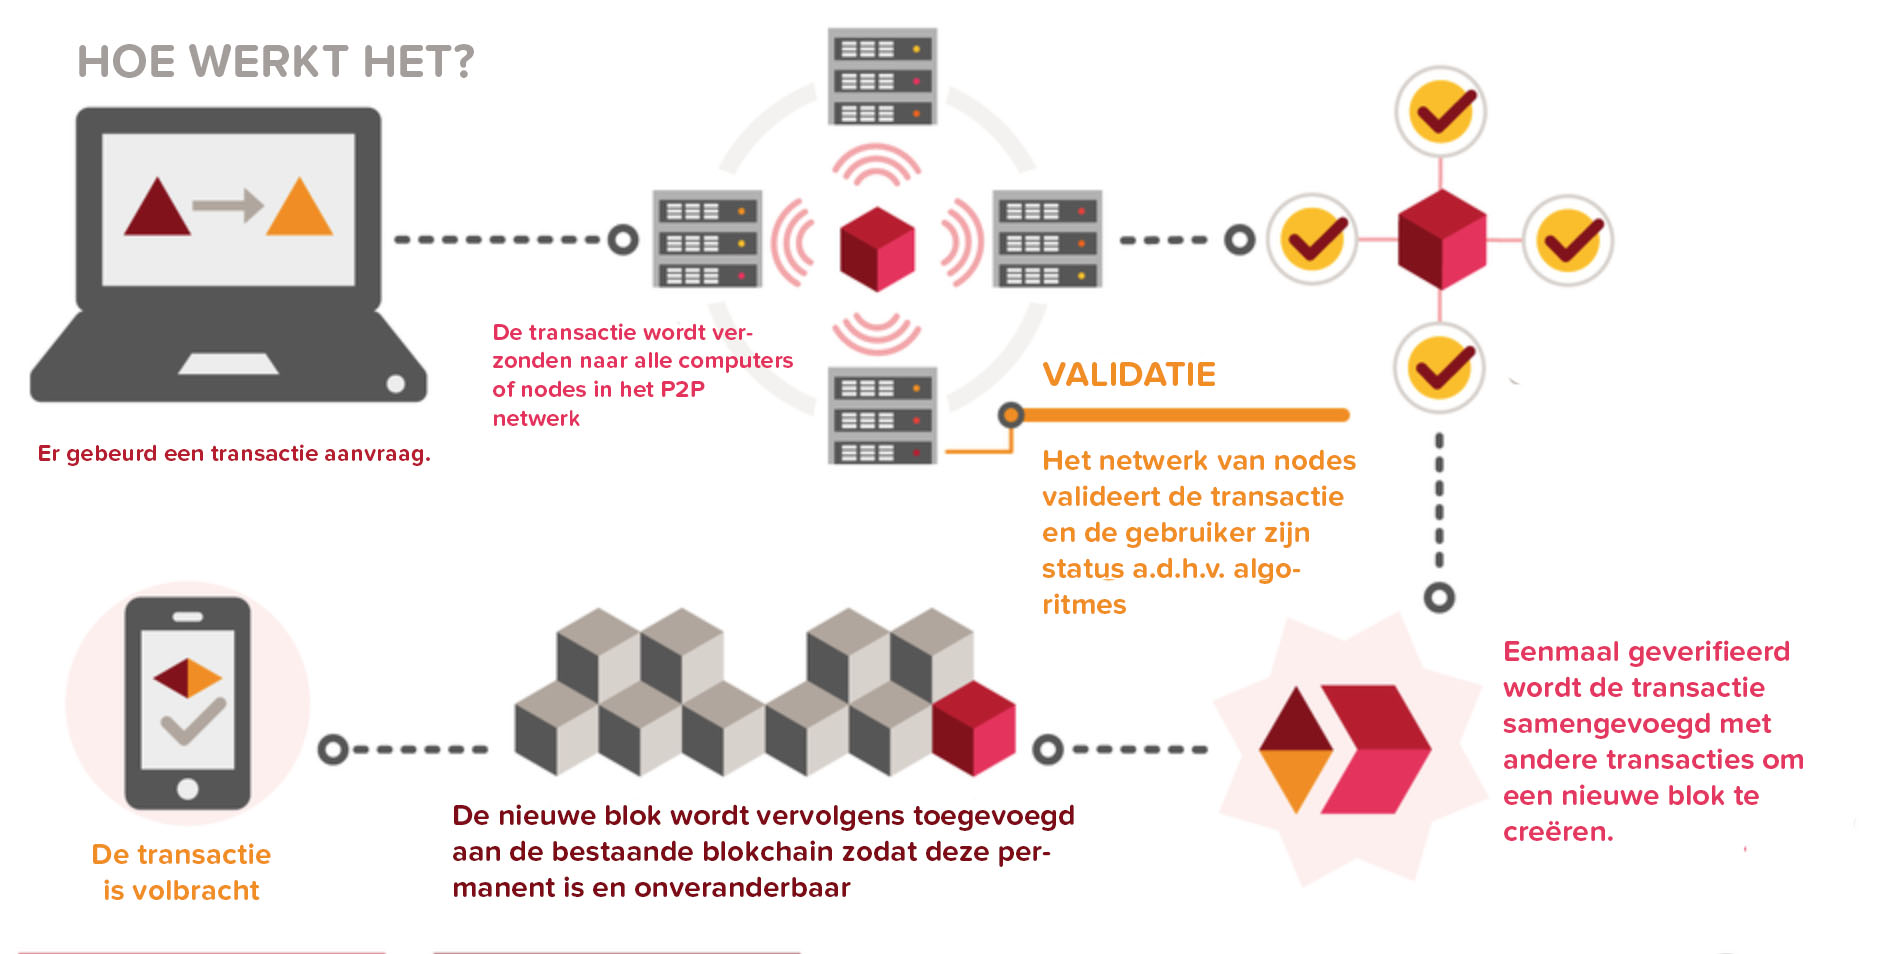
\includegraphics[width=\linewidth]{blockchain-howto.jpg}
	\caption{Grafische voorstelling van de werking van blockchain. Bron: \textcite{pwc.com}}
	\label{fig:blockchain-howto}
\end{figure}

In het algemeen zullen de nodes altijd de langste ``ketting'' aanvaarden als de correcte en zal het verder werken aan deze ketting. Wanneer twee nodes een verschillend blok gaan broadcasten dan kan het zijn dat één node de ene versie eerst zal krijgen en een andere de alternatieve versie eerst zal ontvangen. Daarom zal altijd de eerste dat ontvangen werd gebruikt worden. De alternatieve versie wordt dan bijgehouden. Deze koppeling wordt onderbroken vanaf er een nieuwe proof-of-work wordt gevonden. Hierdoor zal één van de twee versies langer worden en de langste versie zal dan gebruikt worden om op verder te bouwen. De nodes die ondertussen op de andere tak aan het werken waren zullen dan ook overschakelen op deze. Dit wil natuurlijk niet zeggen dat een transactie broadcast alle nodes moeten bereiken, het blijft steeds het internet en een transactie kan verloren geraken. Dit is geen probleem zolang er maar genoeg nodes de transactie ontvangen en deze verifiëren. De nodes die die transactie niet ontvingen zullen dit merken wanneer ze de volgende blok ontvangen en zien dat ze er één hebben gemist en zal deze dan aanvragen aan de andere nodes in het netwerk. De volledige werking is visueel weergegeven op Figuur \ref{fig:blockchain-howto}

Uiteraard kan het ook soms de bedoeling zijn dat bepaalde data niet gezien mag worden op het netwerk. Hiervoor kan gebruik gemaakt worden van enkele cryptografische functies die los gelaten worden op de gegevens en deze versleutelen. Een voorbeeld hiervan en momenteel ook meeste gebruikte algoritme  is sha-256. 

\subsubsection{Wat is SHA-256}
SHA-2 is een verzameling van cryptografische hash functies die gemaakt werden door de National Security Agency (NSA). Wat zijn cryptografische hash functies? Dit zijn wiskundige bewerkingen die kunnen uitgevoerd worden op digitale data. Door vervolgens de berekende ``hash'' te vergelijken met de verwachte hash kan men de data integriteit bepalen. Dit volgens volgend artikel \textcite{Fisher2017} Om een voorbeeld te geven om dit principe te verduidelijken nemen we het volgende voorbeeld. Men heeft een bestand gedownload, laat ons zeggen dat dit een ``word'' bestand is. Men maakt vervolgens een kopie van dit bestand en passen in het word document enkele dingen aan.Vervolgens wordt het document opgeslaan en wordt de hash berekend van beide documenten. Nu heeft men dus het originele bestand en het aangepaste bestand. Als men nu de hash zouden vergelijken van beide documenten dan zal men zien dat deze verschillen. Mocht men nu van de originele versie nog een kopie maken en hiervan de hash berekenen dan zal deze dezelfde zijn van het originele bestand. Op deze manier kan men dus bekijken of een bestand gewijzigd is of niet. Een grafisch voorbeeld van dit voorbeeld is te zien in Figuur \ref{fig:hash-example}.

\begin{figure}
	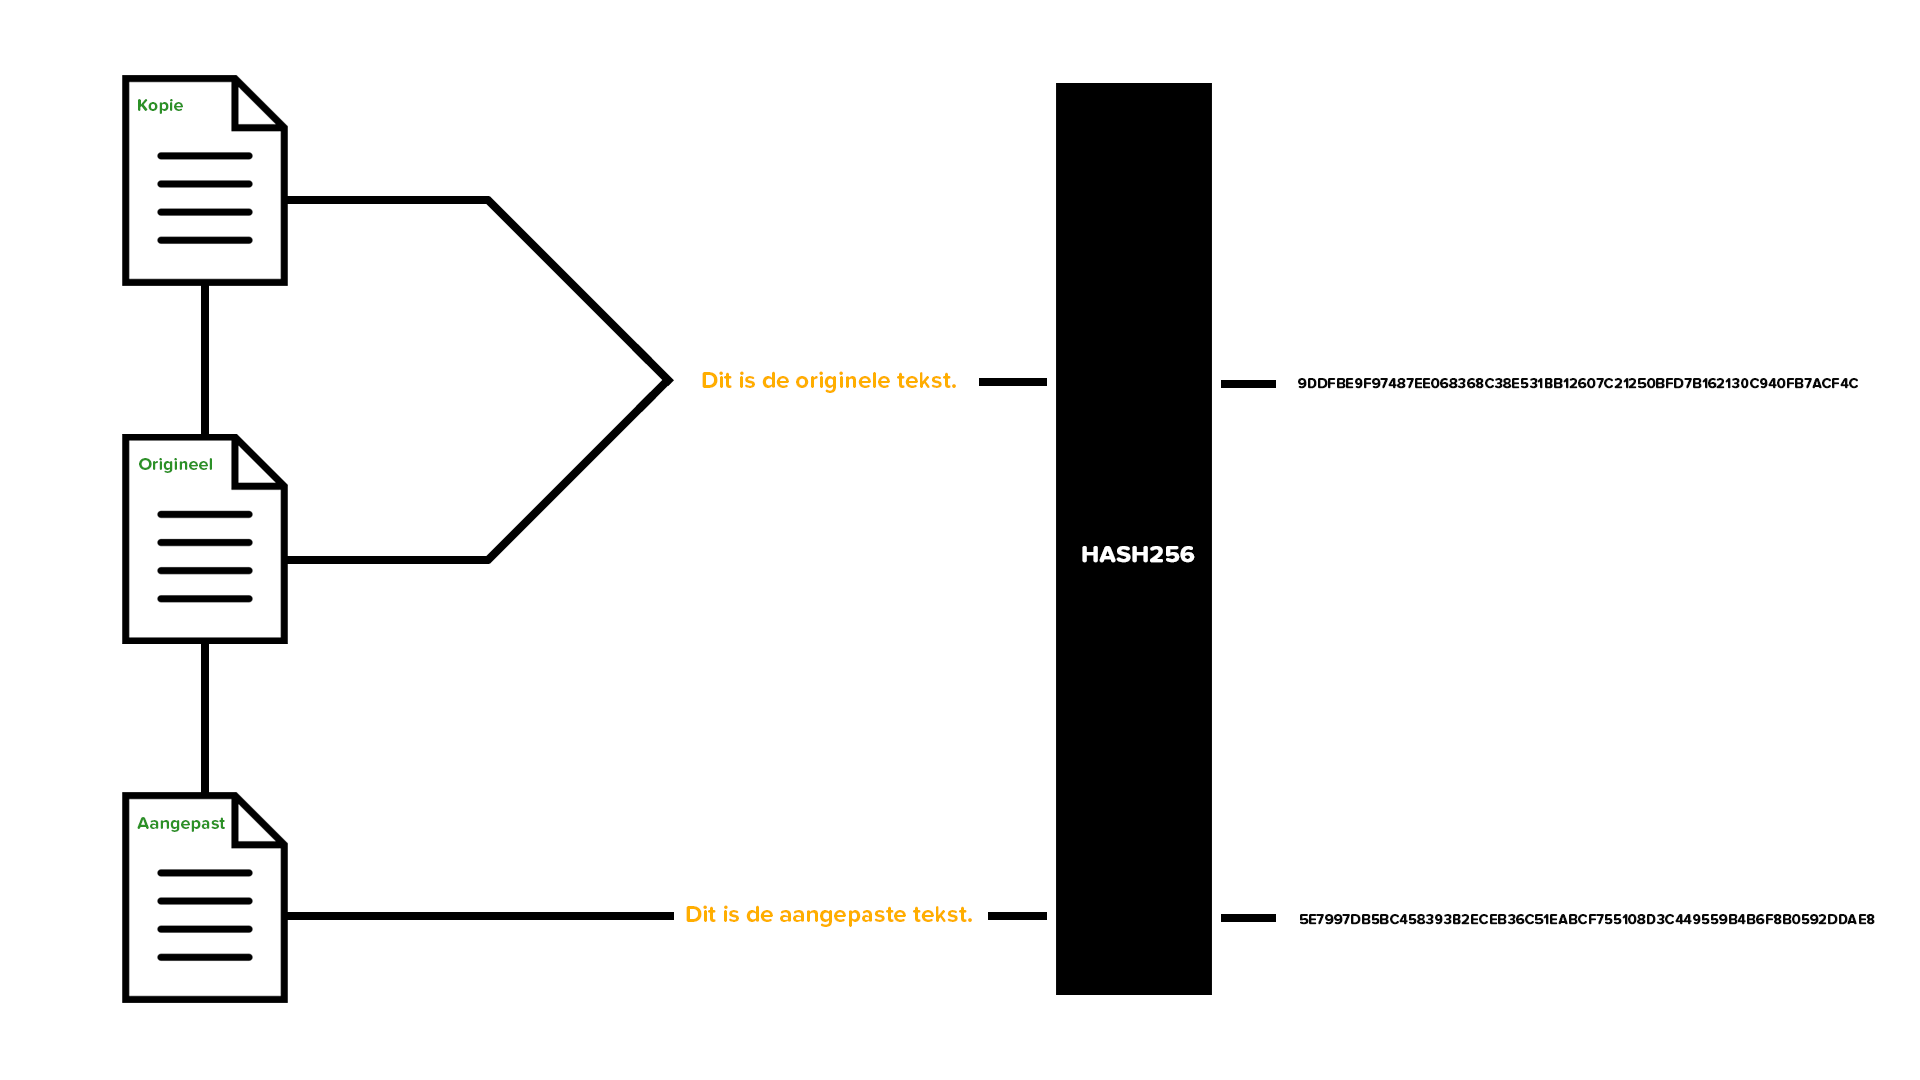
\includegraphics[width=\linewidth]{hash-example.png}
	\caption{Grafische voorstelling van de werking van sha256.}
	\label{fig:hash-example}
\end{figure}

\subsection{Algoritmes}
Er zijn verschillende overeenkomst algoritmes die gebruikt worden voor elk type blockchain. Elk type van algoritme kan ook gebruikt worden in andere types van blockchain maar deze zijn niet altijd even effectief en dit wordt hierdoor meestal ook niet gedaan. De volledige opstelling van blockchain is namelijk volledig naar wens in te stellen. Daarom worden er ook vaak enkele types gedefinieerd die verder aan bod komen.

\subsubsection{Proof-of-work algoritme?}
Proof-of-work is een maatregel die werd ingevoerd om bepaalde aanvallen te voorkomen zoals de gekende denial of service of ook DOS-aanvallen genoemd of om spam op een publiek netwerk tegen te gaan en dit door werk te vragen van de service aanvrager meestal in de vorm van verwerkingstijd door een computer. Proof-of-work kan voorkomen in verschillende vormen, meestal zijn dit wiskundige algoritmen. Enkele voorbeelden zijn puzzels, Diffie-Hellman puzzels, hash sequencies, Merkle tree gebaseerde algoritmen en nog enkele meer. 

Verder zijn er ook verschillende varianten. Deze zijn de Challenge-response en Solution-verification. Het verschil tussen beide kort samengevat komt neer op het volgende, bij challenge-response is de taak die moet uitgevoerd worden nog niet bekend. De server zal deze sturen bij het aanvragen van een service. Bij Solution-verification is de taak op voorhand gekend en kan deze meteen meegestuurd worden met de request. Deze informatie is terug te vinden op  \textcite{Mazieres}. De proof-of-work die Bitcoin zelf gebruikt is bijvoorbeeld gebaseerd op Adam Back's Hashcash, dit volgens \textcite{Nakamoto2008}.

Proof-of-work wordt vooral gebruikt in een publiek netwerk waar geen rechten van toepassing zijn. Iedereen heeft dus evenveel inspraak. Voor andere types van blockchain is dit weer minder van toepassing aangezien de werking niet optimaal zou verlopen. Wanneer men bijvoorbeeld proof-of-work zou gebruiken in een privé netwerk waar alle nodes gekend zijn dan is er weinig nut tot het gebruiken van proof-of-work. Als iemand een aanval probeert te doen op het netwerk dan kan er snel aangewezen worden wie de schuldige was. Proof-of-work zou het geheel ook alleen maar vertragen aangezien er in dit geval telkens een proof-of-work gegenereerd zou moeten worden en dit tijd en CPU-kracht kost. 

\begin{figure}
	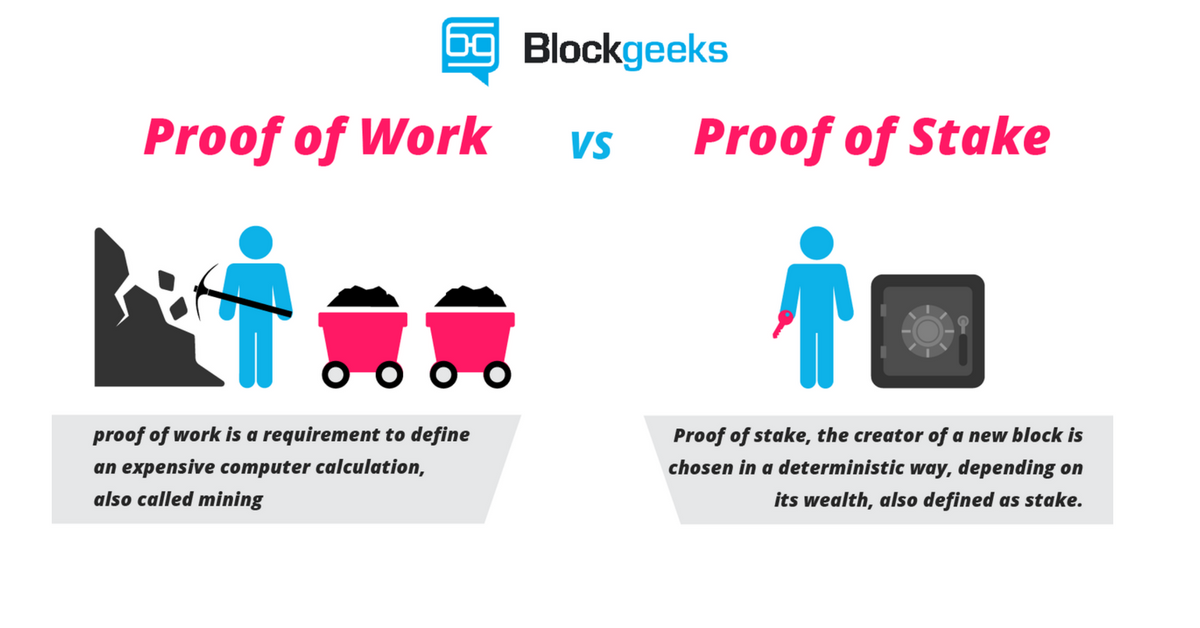
\includegraphics[width=\linewidth]{pow-vs-pos.png}
	\caption{Grafische voorstelling van proof of work tegenover proof of stake. Proof of work heeft dus vooral een hoge kost omdat deze telkens werk moet verichten voor elke transactie die er gebeurt. Dit is een nadeel dat proof of stake niet heeft.  Bron: \textcite{blockgeeks} }
	\label{fig:pow-vs-pos}
\end{figure}

\subsubsection{Proof of stake algoritme}
Wanneer er proof of stake gebruikt wordt om een overeenkomst te bekomen dan wordt er meteen ook vanuit gegaan dat elke node niet meer dezelfde rechten heeft, niet iedereen heeft dus evenveel inspraak meer. Proof of stake werkt volgens het principe dat iemand met meer ``aandelen'' in het netwerk dus ook meer inspraak heeft. Dit heeft als voordeel dat iemand met veel aandelen dus het netwerk niet zal proberen bedriegen aangezien hij deze anders verliest. Het is dus met andere woorden niet de moeite om het netwerk op te lichten en iemand met weinig inspraak of ``aandelen'' heeft ook weer niet genoeg inspraak om het systeem op te lichten. Iemand met veel aandelen zal dus grotere kans hebben om een nieuwe blok aan te maken dan iemand met een kleiner aandeel. Dit volgens \textcite{Buterin2013}. Een grafisch voorbeeld tussen proof of work en proof of stake is te zien op afbeelding \ref{fig:pow-vs-pos}.

\subsubsection{Federated Byzantine Agreement algoritme}
Dit is een methode van overeenkomst die ook gebruik wordt in publieke omgevingen zonder rechten. Natuurlijk moet er ook kunnen getolereerd worden dat er mag gelogen worden of verkeerde informatie mag verzonden worden. Dit noemt met ook wel Byzantine failure. Het is dus vooral belangrijk dat er een overeenkomst tot stand komt ook al werken alle nodes onafhankelijk van elkaar. Er zijn enkele verschillen tussen een Byzantine agreement en een federated Byzantine agreement, het grootste verschil is alvast dat bij een Byzantine agreement alle nodes unaniem moeten overeenkomen. Dit is bij een federated Byzantine agreement anders. Zo kiest hier elke node zelf welke node er vertrouwd wordt en welke niet. Er is dus geen centrale authoriteit gemoeid in het systeem. Nodes kunnen bijvoorbeeld nodes vertrouwen op basis van criteria. Bijvoorbeeld een bank zou als vertrouwbaar kunnen gezien worden, op deze manier kunnen andere nodes herkenning vragen van alle transacties aan deze node. Meestal worden de groeperingen van de nodes overlapt zodat er altijd een algemeen besluit is. Wanneer de nodes niet zouden overlappen dan zou groep 1 van nodes kunnen kiezen voor het ene waar groep 2 zou kunnen kiezen voor het andere. Daarom wordt meestal gebruik gemaakt van een overlapping.

\begin{figure}
	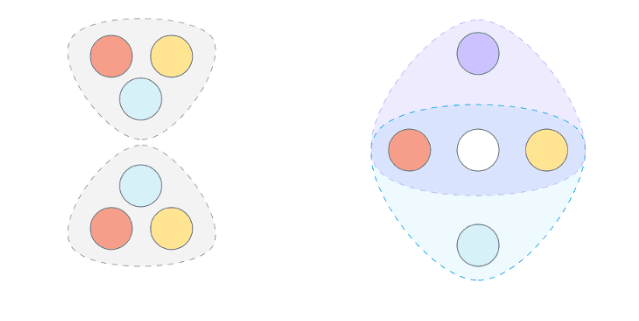
\includegraphics[width=\linewidth]{quorum.png}
	\caption{Een weergave van het verdelen van nodes in groepen. Er zijn verschillende manieren mogelijk van indelen, disjuncte groepen en groepen met een intersectie. Voordelig is om toch een intersectie groep te gebruiken maar dit kan natuurlijk altijd afhangen van de usecase. Het grote verschil tussen beide wordt weergegeven op deze afbeelding. Hier zijn  2 groepen te zien zonder een node die ze gemeen hebben samen met een groep waar enkele nodes wel gemeenschappelijk zijn. Op deze manier wordt er altijd een algemeen akkoord bekomen. Dit kan niet altijd het geval zijn in een disjuncte groep aangezien de ene groep optie 1 kan kiezen terwijl de andere optie 2 kan kiezen en er dus geen algemeen akkoord bekomen wordt. Bron: \textcite{Stellar2015}}
	\label{fig:quorum}
\end{figure}

\subsubsection{Multisignature algoritme}
Als laatste is er multi-sig of multisignature. Deze is er gekomen door één van de problemen die het Bitcoin netwerk tegen kwam en dit was het volgende. Alle bitcoins worden opgeslaan op 1 adres zoals voorheen overlopen, en dit in een wallet. Het nadeel is, iedereen die de privé sleutel heeft tot dit adres heeft ook meteen het recht om transacties uit te voeren en dus het geld over te schrijven. Hierdoor is men opgekomen met multi-sig. Een nieuw type van adres genaamd pay-to-script-hash of afgekort P2SH. Doorheen dit onderwerp wordt dan ook de afkorting gebruiken. Een duidelijk kenmerk van een P2SH adres is dat deze start met een 3. Verder wordt er ook de functionaliteit ondersteund waar er meerdere privé sleutels nodig zijn om een transactie uit te kunnen voeren. Meestal wordt er in de praktijk 2-of-2 of 2-of-3 gebruikt. Dit komt voor bij de werking van een kluis in de bank. De klant heeft hier 1 sleutel en de bank zelf. Dus men heeft beide sleutels nodig om toegang te verkrijgen tot de kluis. Dit komt overeen met een 2-of-2 multi-sig adres. 

Dit heeft meteen ook enkele voordelen wanneer met multi-sig gebruikt. Zo is er geen enkel punt meer van zwakte, hiermee bedoelt men dat wanneer 1 toestel gehackt zou worden dat er nog steeds geen transactie kan plaatsvinden aangezien er een tweede sleutel vereist is. Natuurlijk moet er voor gezorgd worden dat beide sleutels op verschillende toestellen staan en één toestel dus niet beide sleutels heeft. 

\begin{figure}
	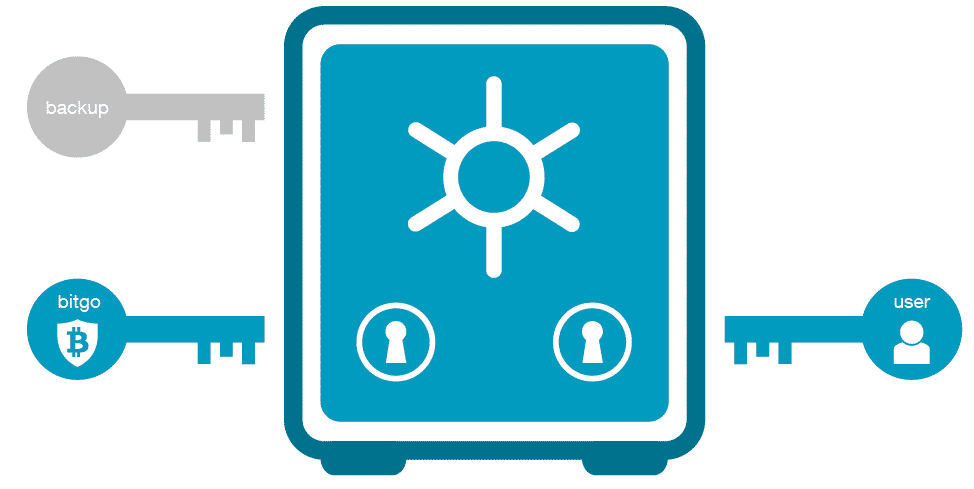
\includegraphics[width=\linewidth]{multisig.png}
	\caption{Een grafische voorstelling van hoe multi-sig werkt. Dit met een voorbeeld van het verdelen van de sleutels en een eventuele backup sleutel indien er gebruik gemaakt wordt van een 2-of-3 opstelling. Bron: \textcite{99bitcoins}}
	\label{fig:multisig}
\end{figure}

Stel dat één van de sleutels zich op een mobiel toestel bevindt en men raakt dit toestel kwijt? 
Dan is dit alweer geen probleem wanneer men gebruik maakt van een 2-of-3 opstelling. Dit wil zeggen dat de gebruiker 1 van de sleutels zelfs mag verliezen omdat er 3 sleutels voorzien zijn die kunnen gebruikt worden. Dit zou kunnen betekenen dat de derde sleutel zich bijvoorbeeld offline bevindt in een ``kluis''. Deze voorstelling is te zien op Figuur \ref{fig:multisig}. Deze overeenkomst strategie heeft dus heel wat mogelijkheden en beveiligen ook het netwerk wanneer één node zou gehackt worden dat er aanvallen op het systeem gebeuren en transacties plaatsvinden met slechte intenties. 

\subsubsection{Round Robin algoritme}
Een ander veel gebruikt algoritme is Round Robin. Dit houdt in dat er willekeurig een node zal worden gekozen. Wanneer een specifieke node gekozen werdt dan wordt deze uitgesloten uit volgende transacties en wordt deze node niet meer toegestaan een blok aan te maken voor een ingesteld aantal transacties. Op deze manier wordt voorkomen dat er voortdurend aanvallen op het netwerk gebeuren aangezien de node willekeurig wordt gekozen. Al wordt een node met slechte bedoelingen gekozen dan zal hij geen poging meer kunnen ondernemen voor de volgende aantal transacties. 

\subsection{Veiligheid}
Blockchain is uitermate veilig, maar een systeem is uiteraard maar zo sterk als zijn zwakste schakel. Wanneer er dus verkeerd wordt omgegaan met deze technologie kan het dus al snel fout lopen. Dit door bijvoorbeeld fouten in code of het onveilig omgaan met data na dit van de blockchain gehaald te hebben. Er zijn dan ook enkele zaken waar streng opgelet moet worden en rekening mee gehouden moet worden. 

\subsubsection{Double spending}
\label{sec:hoeveiligisblockchain}
Wanneer er dus een aanval gebeurt op de blockchain of dus een illegale transactie plaats vindt dan kan deze verworpen worden door de andere servers. In simpele termen komt het er op neer dat zolang de totale CPU capaciteit van de servers groter is dan de capaciteit van de aanvaller dat de blockchain dus veilig is en de aanvallen zal afweren. Dit omdat de aanvaller sneller een alternatieve ketting zou moeten produceren  dan dat de vertrouwde nodes dit doen. Zelf in het geval dat dit zou gebeuren wil dit niet zeggen dat de vertrouwde nodes dit zullen accepteren aangezien dat de aanvaller ook geen waarde kan creëren uit het niets of zichzelf eigenaar kan maken van andere waarden als dit zou bekeken worden in het systeem van Bitcoins. Het enige wat een aanvaller dus in principe kan doen is het aanpassen van zijn eigen transacties, bijvoorbeeld dus geld terug nemen dat hij al eerder uitgaf of ook ``double spending'' genoemd. Verder zijn er natuurlijk nog andere mogelijkheden waar er rekening moet mee gehouden worden op vlak van veiligheid. De kans dat zich dit voordoet is uitermate klein. Zo is te zien in de whitepaper van \textcite{Nakamoto2008}. Stel dat de aanvaller 10 blokken achter zit en de vertrouwde ketting moet inhalen dan heeft deze een kans van 0.0000012\% wanneer men er vanuit gaan dat de aanvaller 10 \% kans heeft om de volgende blok te vinden. Verdere berekeningen zijn te vinden in de paper van \autocite{Nakamoto2008}.

\subsubsection{Andere soorten ``hacks''}
Er zijn uiteraard verschillende manieren van ``hacken'', één van de bekendste is bitcoin mining malware. Dit is malware die verspreid wordt en computers en apparaten infecteert. De geïnfecteerde apparaten worden hierdoor gebruikt om bitcoins te minen wat de toestellen uiteraard zwaar vertragen. 

Andere zaken die veel voorkomen zijn het hacken van de bitcoin wallets, dit zijn bestanden die op de machine staan en die de bitcoins bijhoudt. Deze ``wallets'' bevinden zich op de hardeschijf en kunnen dus gestolen worden. 

Trojans zijn ook bij bitcoin een plaag. Zo zijn er trojans die slechts activeren wanneer er een crypto-currency nummer wordt ontvangen en die deze dan manipuleren zodat de gebruiker bijvoorbeeld geld overschrijft naar de verkeerde persoon. 

Verder zijn er ook nog fouten in de software die bijvoorbeeld toegang geeft tot een blockchain. Blockchain mag in theorie en praktijk nog zo veilig zijn, als er software gebruikt wordt die malfunctioneert dan kan de veiligheid van blockchain ook snel te niet gedaan worden.

Zoals eerder vermeld zijn de transacties of sommige zaken versleuteld voor het publiek. De transactie zelf is zichtbaar maar sommige zaken zijn versleuteld. Wanneer deze encryptie bijvoorbeeld niet sterk genoeg is kan het zijn dat hackers een bepaald deel van de versleutelde tekst toch kan ontfutselen. Blockchain gebruikt in het algemeen een SHA-256 versleuteling, deze wordt onder andere ook gebruikt voor het versleutelen van HTTPS en dergelijke. Wanneer deze encryptie zou falen zou niet enkel blockchain dus een zwaar probleem hebben. Onderzoekers bevestigden wel dat SHA-256 zeker sterk genoeg is om zaken te beveiligen voor een hele tijd.

\subsection{Automatisering}
Op sommige systemen is zelf rekening gehouden met automatisering. Zo is het bijvoorbeeld mogelijk om bepaalde taken automatisch te laten gebeuren wanneer er aan bepaalde criteria wordt voldaan. Een goed voorbeeld hiervan zijn smart contracts.

\subsubsection{Smart contracts}
Wat zijn Smart contracts? Dit zijn computer protocols die bedoeld zijn om het toepassen van een contract te vereenvoudigen en te verifiëren. De bedoeling van smart contracts is om bepaalde zaken te kunnen coderen die dan later automatisch kunnen uitgevoerd worden. Een grafisch voorbeeld is te vinden in Figuur \ref{fig:smartcontracts}. De scripts zijn vooral populair op de Ethereum blockchain (een andere cryptocurrency) en worden hier ook wel dapps genoemd of decentralised applications. Een populaire programmeertaal voor het maken van smart contracts is dan ook ``Solidity''. Deze scripts worden dan opgeslaan in de blockchain zodat ze later kunnen uitgevoerd worden door de EVM (Ethereum Virtual Machine). Dit volgens \textcite{Chandrayan2017}.

 \begin{figure}
	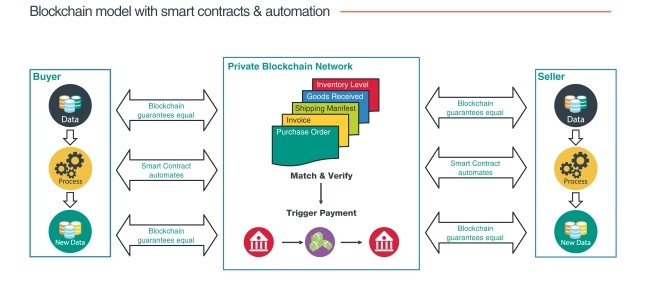
\includegraphics[width=\linewidth]{smartcontracts.jpeg}
	\caption{Grafische voorstelling van de werking van smart contracts. Men zien de aankoop van een product. Vervolgens ziet men dus dat éénmaal aan alle voorwaarden wordt voldaan dat het smartcontract wordt uitgevoerd en dat de betaling in werking wordt gezet. Er wordt dus een bepaalde taak geautomatiseerd bij het voldoen van enkele voorwaarden die op voorhand worden ingesteld met bevoorbeeld een scripting/programmeer-taal zoals Solidity. Bron: \textcite{Itweb}}
	\label{fig:smartcontracts}
\end{figure}


\section{Verzekeringen en unieke documenten}
\subsection{Wat is een verzekeringsagent en een verzekeringsmakelaar?}
Een verzekeringsagent is een gebonden tussenpersoon. Dit wil zeggen dat deze persoon voor één verzekeringsmaatschapij werkt, dit verschilt van een verzekeringsmakelaar die onafhankelijk is en niet gebonden is aan één verzekeringsmaatschapij. Een verzekeringsagent kan dus slechts de verzekeringen aanbieden van zijn eigen maatschapij waar een verzekeringsmakelaar verzekeringen kan aanbieden van verschillende maatschapijen. 

Er zijn uiteraard meerdere benamingen voor een verzekeringsagent die allemaal op hetzelfde neerkomen zo wordt een verzekeringsagent bijvoorbeeld ook een tussenpersoon genoemd, een intermediair of een financieel adviseur. 

\subsection{Wat doet een verzekeringsagent of verzekeringsmakelaar?}
Zoals eerder vermeld doet een verzekeringsagent en verzekeringsmakelaar juist hetzelfde. Het enige verschil tussen beide is dus dat een verzekeringsagent gebonden is aan één maatschapij waar een verzekeringsmakelaar dit niet is. Voor vereenvoudiging doorheen dit document zal ik steeds verwijzen naar een verzekeringsmakelaar. 

Wat doet een verzekeringsmakelaar nu juist? Een verzekeringsmakelaar zal jouw wensen en vragen allemaal noteren en zal dit gebruiken om de voor u zo optimale verzekering te vinden. Nadien overloopt deze dan alle mogelijkheden met de nodige uitleg. Verzekeren kan een zeer complex iets zijn en dan is een verzekeringsmakelaar zeker nuttig om te raadplegen. Dit alles is te vinden in volgend document \textcite{Verzekeruzelf.nl}.

\subsection{Soorten verzekeringen en verzekeringsdocumenten}
Er zijn heel veel soorten verzekeringen. Zo kan in theorie alles verzekerd worden al is dit niet altijd gebruikelijk. In volgend document \textcite{verzekeringen.com2015} zijn enkele voorbeelden van beroemdheden die verschillende lichaamsdelen lieten verzekeren te vinden want ook dit is uiteraard mogelijk. Bijvoorbeeld wanneer een gitarist zijn hand zou verliezen dan verliest deze hiermee ook meteen de mogelijkheid tot het uitoefenen van zijn beroep. Er zijn dus heel wat mogelijkheden beschikbaar, volgens het volgende artikel \textcite{BFOverzekeringen} van de Belgische overheid zijn dit de meest voorkomende verzekeringen.

\begin{itemize}
	\item Autoverzekering
	\item Brandverzekering en natuurrampen
	\item Familiale BA-verzekering
	\item Rechtsbijstand
	\item Ziekte- en hospitalisatieverzekering
	\item Reisverzekering
	\item Vrijwilligersverzekering
	\item Schuldsaldoverzekering
	\item Levensverzekering of overlijdensverzekering
	\item Verzekeringen in specifieke situaties
\end{itemize}

Voor elk van bovenstaande verzekeringen is er dus een contract, dit bijgevolge ook uniek zal zijn en bepaalde voorwaarden zal bevatten. Documenten zoals deze zouden dus perfect in een blockchain kunnen opgeslagen kunnen worden. 

\subsection{Is verzekeren verplicht?}
Er wordt inderdaad ook onderscheid gemaakt tussen verplichte verzekeringen en niet verplichte verzekeringen. Zo kan men verplicht zijn een verzekering te nemen om een bepaalde activiteit te mogen uitvoeren. Denk maar aan een BA verzekering, wanneer een wagen niet verzekerd is dan kan deze niet in verkeer worden gebracht. Daar tegenover is een bestuurdersverzekering geen verplichte verzekering. Ook voor het uitvoeren van bepaalde beroepen is het verplicht om een verzekering aan te gaan. Enkele voorbeelden zijn architecten, boekhouders, belastingsconsulenten en nog vele meer. Sommige verzekeringen kunnen dan weer wel contractueel verplicht worden. Zo kan een huisbaas bijvoorbeeld de huurder verplichten een brandverzekering af te sluiten. Dit volgens het volgende artikel van \textcite{BFOverplichteVerzekeringen}. 

%%\lipsum[7-20]

\section{Probleemstelling en Onderzoeksvragen}
\label{sec:onderzoeksvragen}

%% TODO:
%% Uit je probleemstelling moet duidelijk zijn dat je onderzoek een meerwaarde
%% heeft voor een concrete doelgroep (bv. een bedrijf).
%%
%% Wees zo concreet mogelijk bij het formuleren van je
%% onderzoeksvra(a)g(en). Een onderzoeksvraag is trouwens iets waar nog
%% niemand op dit moment een antwoord heeft (voor zover je kan nagaan).

Het de bedoeling om het gehele systeem toegankelijk te maken voor de vereiste instanties. Denk maar aan de overheid, verzekeraars, garages indien het gaat over een autoverzekering, agenten en vele meer. 

Het probleem dat zich momenteel voordoet is dat er een hele hoop documenten nodig zijn en de communicatie tussen verschillende partijen een hele tijd kan duren.

Denk maar aan de situatie wanneer er een verkeersongeval gebeurt. Er moeten een schadeforumulier worden ingevuld en beide partijen hebben een versie nodig. Vervolgens moet dit worden doorgestuurd naar hun persoonlijke verzekeraar die op hun beurt contact moeten opnemen met elkaar. Er wordt bij beide partijen dan ook een schadedocument opgemaakt. Vervolgens moet er ook een inspectie gebeuren van het voertuig om de schade op te meten. Hiervoor wordt door deze partij nog enkele documenten opgemaakt. Dit document wordt dan uiteindelijk naar beide partijen verstuurd. Al deze documenten zijn echter verspreid en worden beheerd door verschillende partijen. Hierdoor onstaat er ook heel veel communicatie en vaak ook miscommunicatie. Zo weten de slachtoffers nooit hoe ver de zaken staan en is er vaak een lange wachttijd. 

Blockchain zou hier een uistekende oplossing voor zijn om alle documenten en communicatie te verrichten op deze manier. Waaruit ook volgende onderzoeksvragen voortkomen.
\begin{itemize}
	\item Hoe kan men blockchain toepassen op verzekeringsdocumenten en een eco-systeem opbouwen voor meerdere partijen?
	\item Hoe kan men blockchain gebruiken om oplichting van verzekeringen tegen te gaan.
\end{itemize}

\section{Opzet van deze bachelorproef}
\label{sec:opzet-bachelorproef}

%% TODO: Het is gebruikelijk aan het einde van de inleiding een overzicht te
%% geven van de opbouw van de rest van de tekst. Deze sectie bevat al een aanzet
%% die je kan aanvullen/aanpassen in functie van je eigen tekst.

De rest van deze bachelorproef is als volgt opgebouwd:

In Hoofdstuk~\ref{ch:methodologie} wordt de methodologie toegelicht en worden de gebruikte onderzoekstechnieken besproken om een antwoord te kunnen formuleren op de onderzoeksvragen.

In Hoofdstuk \ref{ch:add-to-blockchain} wordt onderzocht hoe data kan worden toegevoegd aan een blokchain. Verder wordt onderzocht welke zaken van de transactie afgeschermd moet worden om breuken op de privacy te voorkomen. 

In Hoofdstuk \ref{ch:eco-system} wordt een systeem gebouwd aan de hand van de verschillende types van blockchain. Hier worden meteen ook de mogelijke algoritmen toegepast en besproken  en vervolgens ook vergeleken met elkaar. Verder worden de voor- en nadelen meteen weergegeven. 

In Hoofdstuk \ref{ch:usecases} worden enkele usecases opgelost met blockchain en worden duidelijk vereenvoudigd door gebruik van blockchain. 

In Hoofdstuk \ref{ch:alternative-technology} wordt vervolgens een alternatieve technologie besproken en wordt onze onderzoeksvraag uitgewerkt met deze technologie. Ook van deze technologie zullen de voordelen en eventuele nadelen aangekaart worden. 

In Hoofdstuk~\ref{ch:conclusie}, tenslotte, wordt de conclusie gegeven en een antwoord geformuleerd op de onderzoeksvragen. Daarbij wordt ook een aanzet gegeven voor toekomstig onderzoek binnen dit domein.

